\section{Proof of Concept Implementation}\label{ch:implementation}
% +Implementation:
% *System:
% 	-Raspbian OS: distro de debian para Raspberry Pi, que se describirá en los tests
% 	-LEDE: ash terminal (shell command interpreter), POSIX, typical hardware, libraries with no hardware aceleration vs smart card MULTOS,
%
% *Delegation
%  -REST as current delegation protocol: curl script bash
%  -BIOSC as current APDU transmission protocol: no security -> no overload.
% *Smart Card
%  
%  -IoT Smart Card software design and implementation notes.
%  -Sequence diagrams. TODO


This section presents the first PoC implementation, introducing the IoT system used in the tests, the delegation protocols, one for the computation offloading of the IoT device on the P2ABCE server, and another one for the transmission of APDU Commands, and finally, the IoT smart card implementation.

The PoC is developed under a Linux based system aimed for IoT environments, a fork of OpenWrt, called LEDE (Linux Embedded Development Environment), that will serve as a starting point for future implementations in more constrained devices or different systems. 
The delegation server we will run on Raspbian OS, in a Raspberry Pi 3, with a working Java Runtime.


%%%Regarding the definition of the P2ABCE API, it is a work in progress, and in the meantime,         we           will work with the REST API currently available in the P2ABCE project to perform the delegation. Regarding the \textit{IoT Smart Card}, the P2ABCE project defines the APDU instructions with the corresponding format of the APDU Commands and Responses. In the next section we will explain the PoC for IoT based on these P2ABCE specifications.


%\subsection{PoC Delegation}

\hfil

The delegation process has two steps, first the IoT device calls the P2ABCE server to offload the parsing of the XML data, and then the P2ABCE server, sending APDU Commands, delegates to the IoT smart card the cryptographic calculations.


\subsection{Delegation to P2ABCE Server}


Currently P2ABCE offers multiple REST web services to run different roles in P2ABCE system: User Service, Issuer Service, Verification Service, etc. 
%Any third party application that integrates P2ABCE with their system can make use of these services or implement the functionality using the library written in Java, the tool that the REST services actually use.
%
%In this PoC, the P2ABCE's User Service needed to be modified, because this is the role the IoT device plays. We added the following REST call:
%\begin{center}
%	\textit{/initIoTsmartcard/{issuerParametersUid}?host=\&port=}
%\end{center}
%where we communicate the P2ABCE server that an IoT Smart Card is accessible via the IP address \textit{host} and TCP port \textit{port}.
After an analysis of P2ABCE's code, the \texttt{HardwareSmartcard} class implements the \texttt{Smartcard} interface using the package of abstract classes \texttt{javax.smartcardio} to communicate with the physical smart cards. The Oracle JRE implements these package for the majority of smart card manufacturers. For our PoC, we implement the \texttt{javax.smartcardio} package so it transmits the APDUs with our custom protocol, making the use of a physical or IoT smart card totally transparent to the \texttt{HardwareSmartcard} class, enhancing maintainability, and following the \textit{expert pattern} from the known GRASP guidelines.

In this PoC, the P2ABCE's User Service was modified to add a new method receiving the IoT device's  IP address and a port where the IoT Smart Card will be listening for the APDU Commands.
This method creates a new \textit{HardwareSmartcard} object, but instead of the \textit{javax.smartcardio} Oracle's \textit{CardTerminal} implementation, we use our own \textit{IoTsmartcardio} implementation for the \textit{HardwareSmartcard} constructor.


The remaining REST methods are left untouched, and will serve to parse the XML files exchanged.

\hfil

\subsection{APDU Dialogue Transmission}


To transmit the APDU messages in our PoC we use a simple protocol, that we will refer as BIOSC (Basic Input Output Smart Card). It consists on one byte for the instruction, that can mean either an APDU Commnad or a finishing instruction to close the connection.

In the first case, the header continuous with two more bytes for the length of the payload bytes to read, which are the APDU Command bytes.
To send an APDU Response in BIOSC, the IoT device sends back to the server two bytes for the length and then the raw APDU Response bytes. The messages are sent over TCP for a reliable transmission.

We lack any security (authentication or authorization) that a real system should implement. It is vital to authenticate the delegation service, to authorize it to perform APDU Commands, and the same with the IoT device, to prevent impersonation attacks. But using BIOSC for the transmission of the APDU messages in the PoC, with only 3 bytes of overhead, helps us in the  benchmarks to measure the real performance of the system.


\subsection{IoT Smart Card Implementation}

In this section we present the code architecture and sequence diagram of the IoT Smart Card PoC, based on ABC4Trust's Card Lite.

\hfil

\textsc{Code structure}
We divide the project in three different sections with the objective of enhancing maintainability, improving future changes, ports, fixes, etc.
In \autoref{fig:IoTCScomponents-bw} we show how the project is structured in three sections:

%\begin{figure}[bth]
%	\begin{center}
%		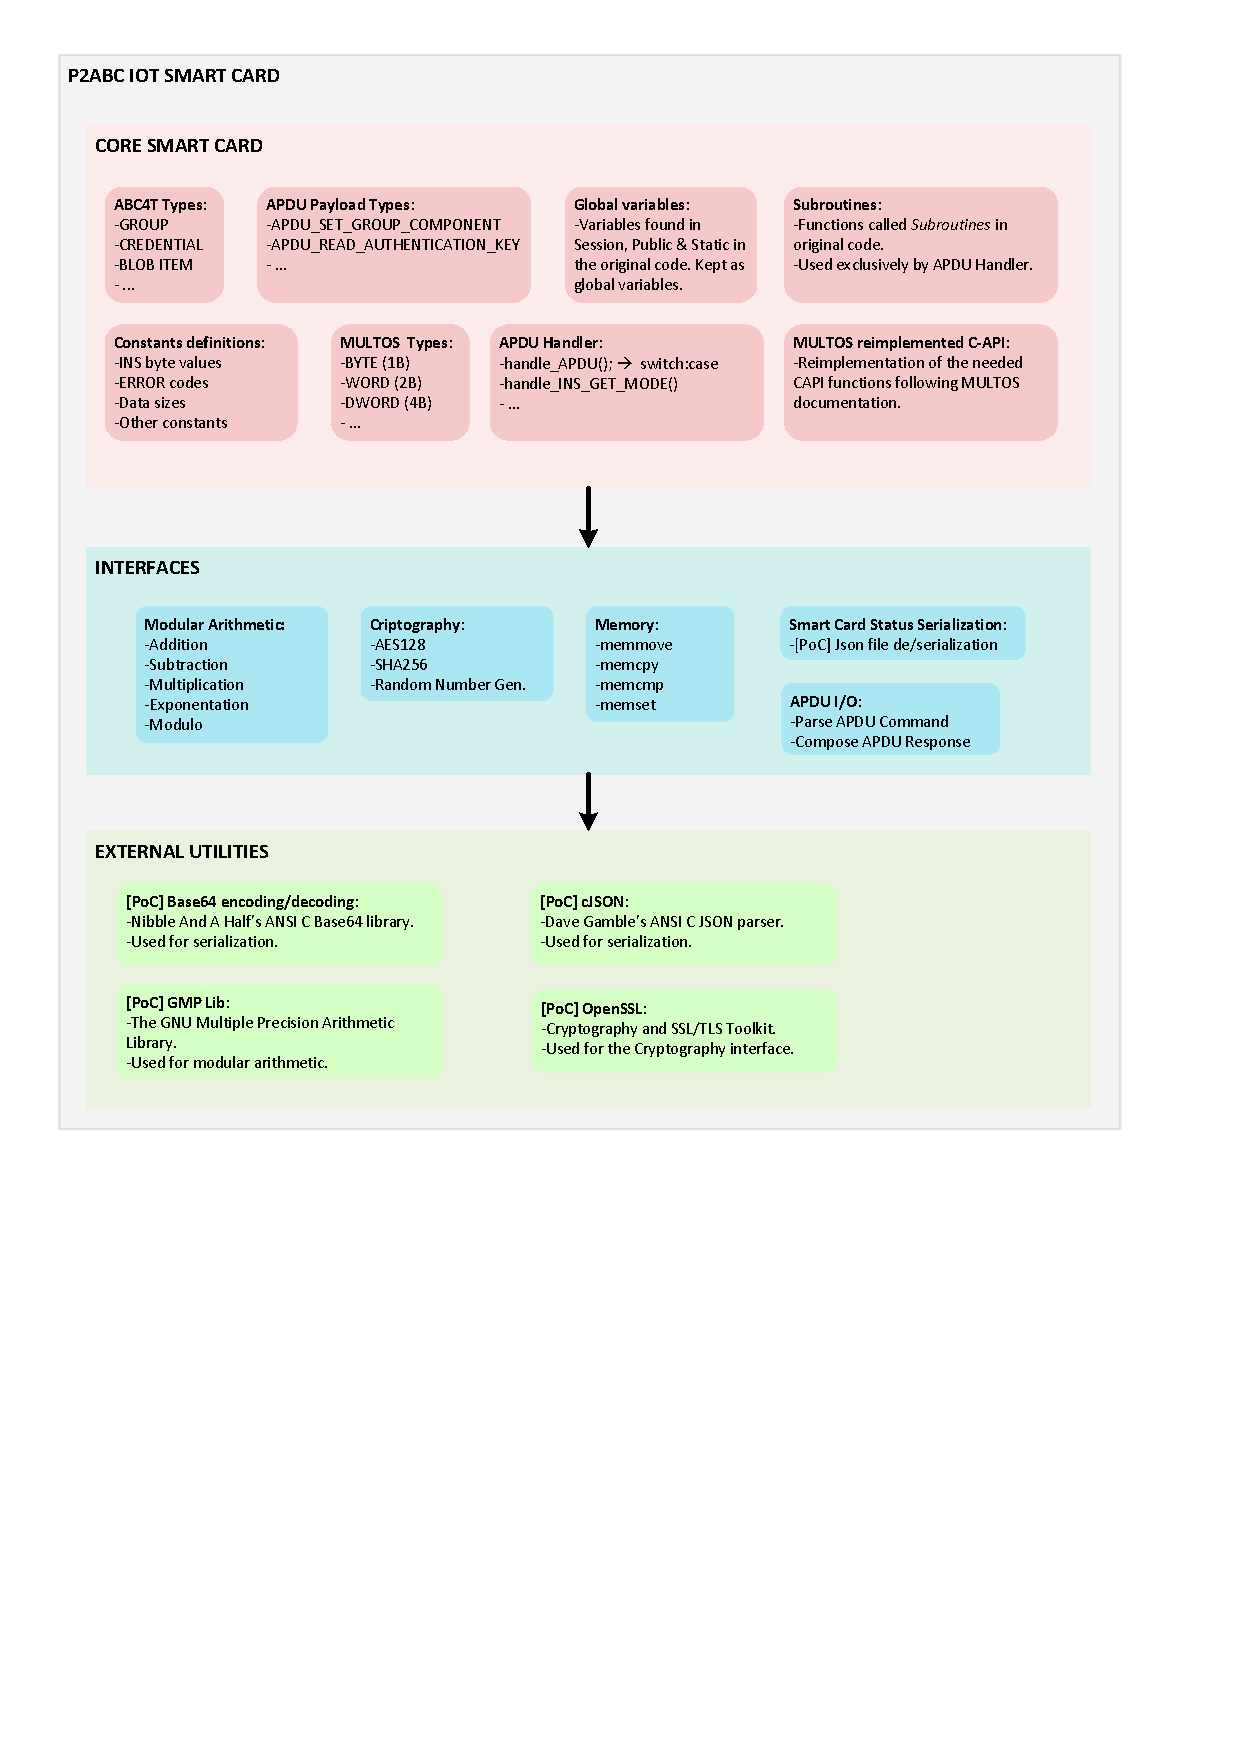
\includegraphics[width=\linewidth]{gfx/IoTCScomponents-color}
%	\end{center}
%	\caption{IoT Smart Card Code Structure.}
%	\label{fig:IoTCScomponents-color}
%\end{figure}

\begin{figure}[bth]
	\begin{center}
		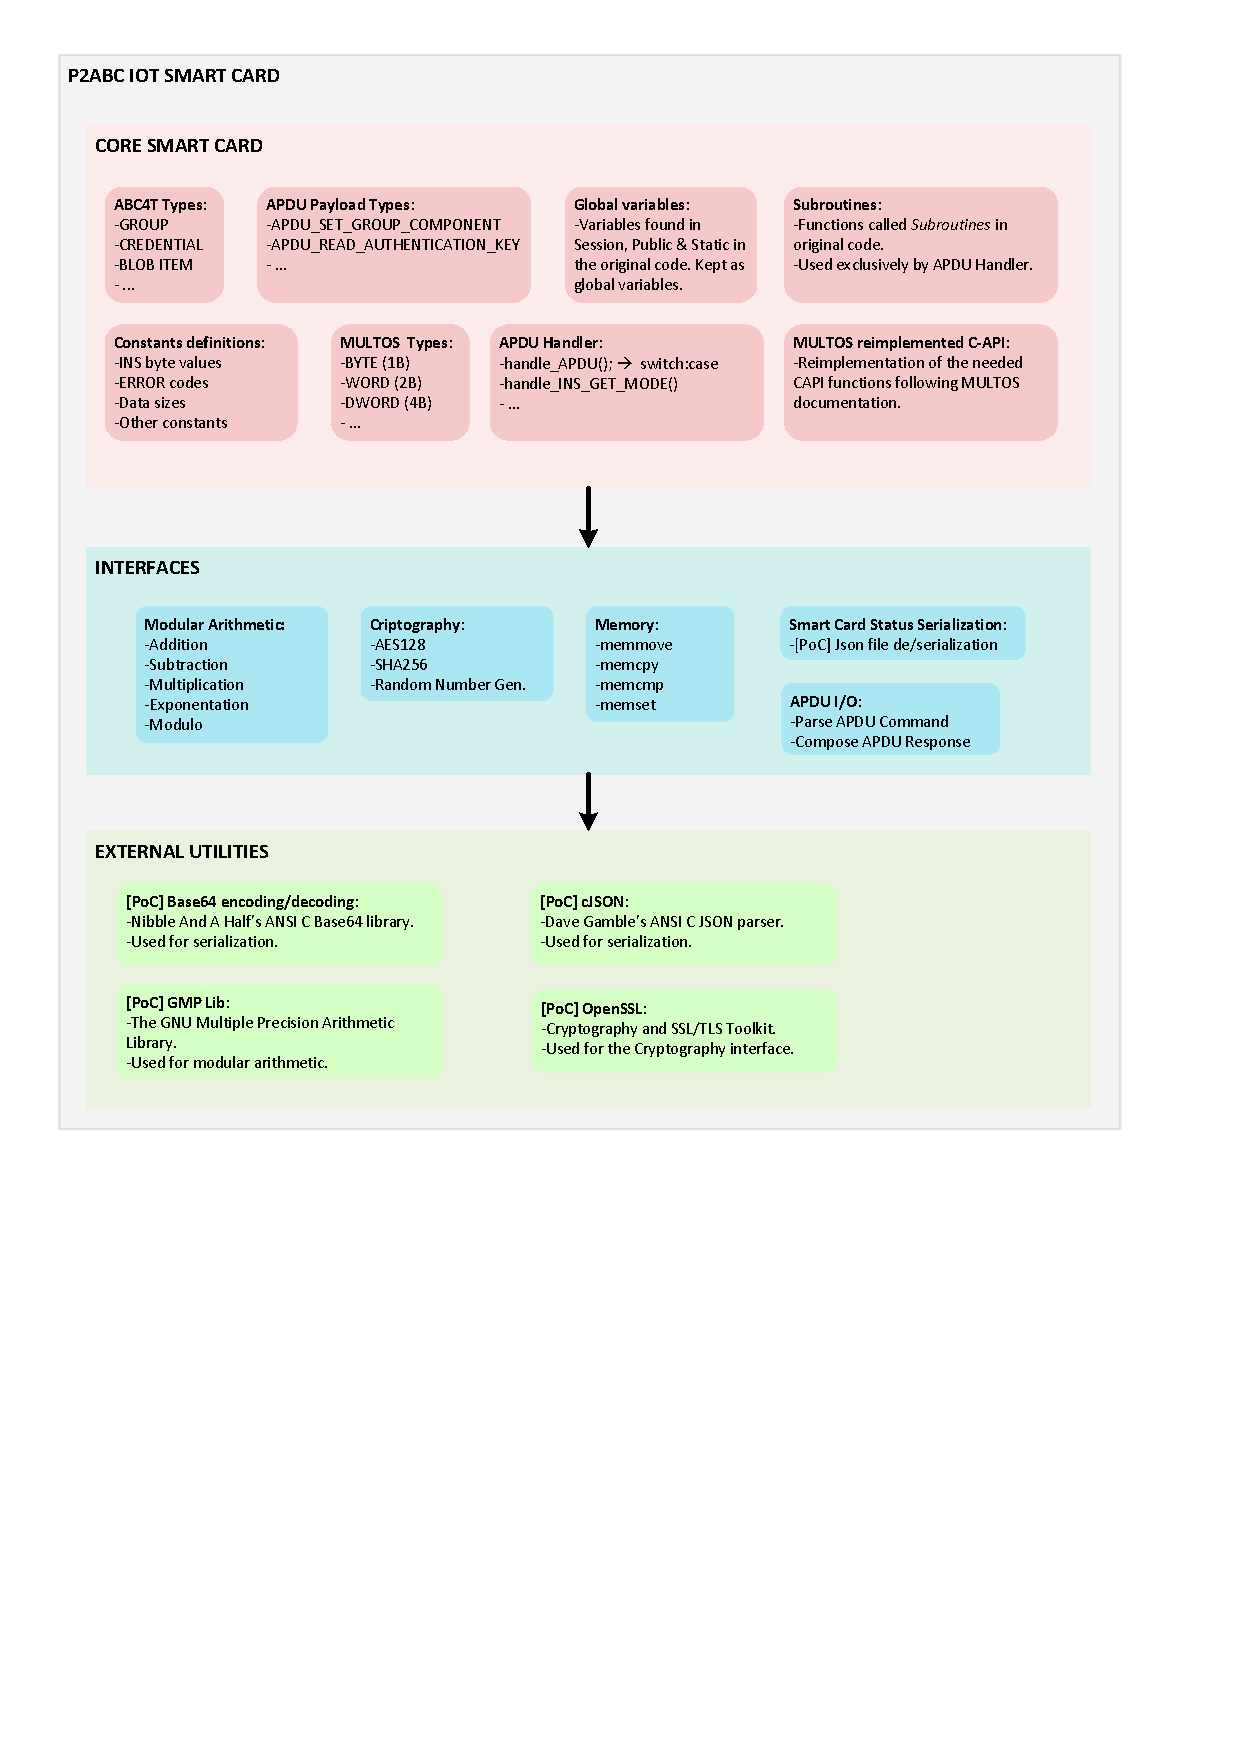
\includegraphics[width=\linewidth]{gfx/IoTCScomponents-color}
	\end{center}
	\caption{IoT Smart Card Code Structure.}
	\label{fig:IoTCScomponents-bw}
\end{figure}


\hfil

\textbf{Core smart card:} The smart card logic lies here, with the concepts of APDU Commands, the instructions that are defined for P2ABCE smart cards, and how to process them and generate proper APDU Responses.

Here we adapted the ABC4Trust Card Lite's code. However, the ABC4Trust's code heavily depends on the MULTOS platform, therefore, we reimplement the used MULTOS functions following the documentation, adapting it in some cases for \textit{expanded functionality}, to avoid some MULTOS API limitations, like in \cite{vullers2013efficient}, when they noted that MULTOS' \texttt{ModularExponentiation}  function does not accept exponents larger than the modulus size, so they implemented \texttt{SpecialModularExponentiation}.

MULTOS compiler does not apply data structure alignment. This affects the inherited ABC4Trust's code because of the use of \texttt{memcpy} to copy multiple variables in one call.%, for example, the APDU Command payload usually includes multiple data, and instead of copying one variable at a time, the \texttt{struct} is defined with the same order and copies everything at once.

The temporal solution is to use \texttt{struct \_\_attribute\_\_((\_\_packed\_\_))} to ask a GCC compiler to not use padding in the structs, but this is not standard, neither a good practice. A deeper refactorization of the code is needed where the hidden copies of variables must be made explicit, letting the compiler manage the memory layout on its own.

\hfil

\textbf{Interfaces:} To reimplement some of the MULTOS functions, we defined a facade to isolate the implementation of the core smart card from our different options, that could vary depending on the hardware or the system used by the IoT device.
With this facade we could, for example, change the implementation of cryptographic functions with a hardware implementation (e.g. Atmel's chips for SHA and AES), or software implementations optimised for the target platform.

The interfaces defined can be organized in 5 groups (see \autoref{fig:IoTCScomponents-bw}), depending on their purpose: Modular Arithmetic, Cryptography, Memory Management, Serialization and APDU Parsing.

\hfil

\textbf{External utilities:} In our PoC we used two ANSI C libraries, for base64 and JSON, and two shared libraries available as packages in LEDE: GMPLib and OpenSSL. These libraries use dynamic memory and offer more functionality than we need, and although they are useful tools for the early development versions of the PoC, future versions should use more lightweight solutions.

\hfil

The \textit{interfaces} and \textit{external utilities} sections  allow that the project is easily ported to specific targets without modifying the smart card logic.


\hfil

\textsc{Execution workflow}

The sequence diagram from \autoref{fig:sequenceBIOSC} shows the execution of the PoC IoT smart card.



\begin{figure*}[bth]
	\begin{center}
		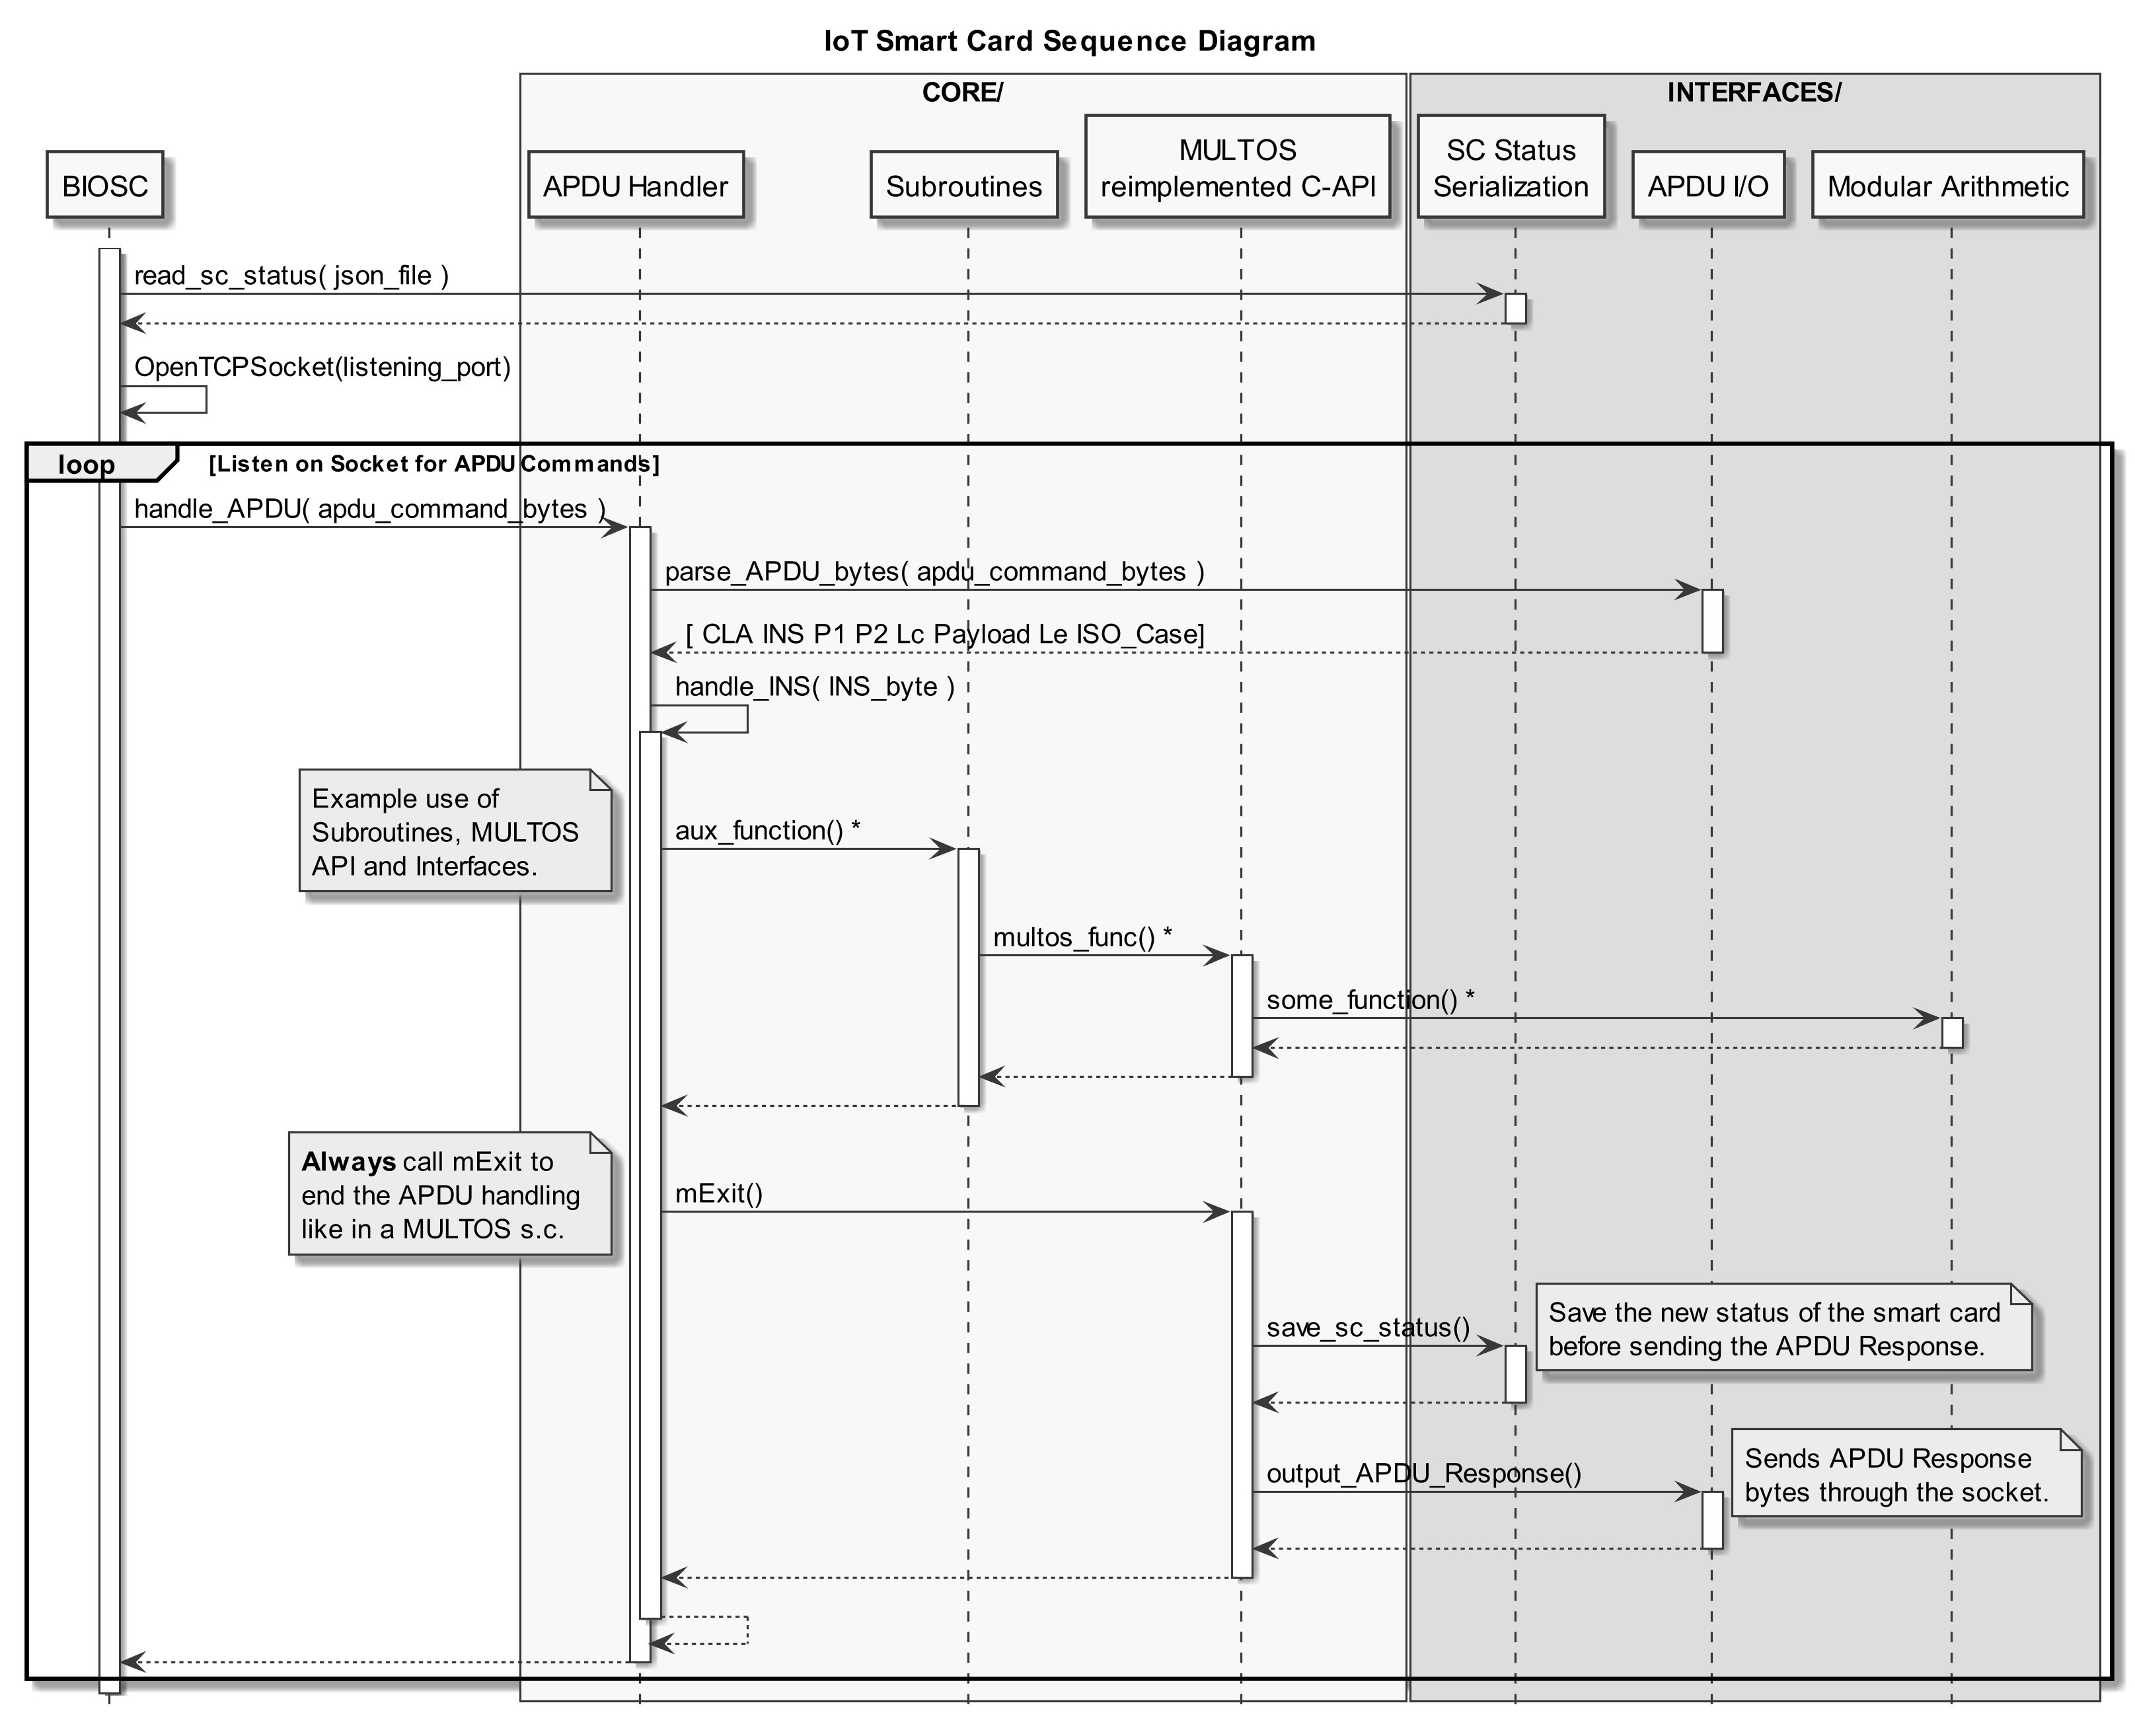
\includegraphics[width=0.8\textwidth]{gfx/UML/sequenceBIOSC}
	\end{center}
	\caption{IoT Smart Card Sequence Diagram.}
	\label{fig:sequenceBIOSC}
\end{figure*}



The program starts with the \texttt{main} function in BIOSC, that deserializes the status from the Json file, and listens on a loop for APDU Commands from the delegation server.

Every time an APDU Command arrives, it calls the function \texttt{handle\_APDU()} with the raw APDU bytes. The Handler calls the APDU I/O interface to parse the bytes, storing in global variables the APDU structure. Using a \texttt{switch-case} expression on the \texttt{INS} byte, the Handler calls an \textit{Instruction handler} function.

Inside this function, it may call multiple functions from the Subroutines, that may call MULTOS C-API functions, which, in turn, may use an interface to perform its functionality.

Finally, every instruction handler must end, before the \texttt{return;} expression, with a call to \texttt{mExit}. This reimplemented MULTOS function will save the current status of the smart card and send the APDU Response back to the delegation server.

After returning from these functions, \texttt{mExit}, the instruction handler and the APDU handler, the program listens again from the socket.


